\section{RQ8: Runtime and Lifecycle Value}
\label{sec:economics}

NDC is implementation-independent search work; elapsed time is the deployment endpoint. We therefore report both without substituting one for the other.

\paragraph{Measured fixed-machine runtime.}
The historical timing campaign covers the registered 24-build Faiss panel per dataset on the machine described in Section~\ref{sec:methodology}. The original sub-millisecond per-cell CV criterion was rejected before policy gains were inspected; the supplement records why an amended action-block stability gate was sealed before gain mapping. Source one-rung reduces wall time by 9.44 [9.04, 9.77]\% on SIFT and 26.04 [25.62, 26.44]\% on Arxiv. p95 ratios are 0.988 and 0.914, and minimum LOTO reductions are 9.42\% and 25.97\%. These conservative 24-build estimates and the larger prospective-panel estimates use different build/query panels. The prospective confirmation and paired audit retain positive reductions on disjoint query roles evaluated over the same eight-build panel; they are not independent build replications.

\paragraph{Lifecycle accounting.}
For policy $\pi$ at horizon $N$,
\begin{equation}
 C_\pi(N)=C_{{\rm acquire},\pi}+N\bar c_\pi,
 \qquad N_{\rm BE}=\frac{\Delta C_{\rm acquire}}{\bar c_{\rm end}-\bar c_\pi}.
 \label{eq:breakeven}
\end{equation}
Cached history treats old profiles and truth as sunk; cold history charges their acquisition once per snapshot. Target selection, candidate and endpoint certification, and exact target truth are charged to recovery; truth is modeled as one scan of 100,000 vectors per labeled query. At $N=10^6$, cold-history joint-error TCP saves about 490 million NDC on SIFT and 389 million on Arxiv; break-even is approximately 396,000 and 457,000 executions, compared with 129,000 and 148,000 under cached history. Four Arxiv fallback targets do not individually amortize positive recovery overhead.

\begin{table}[t]
\caption{Joint-error TCP break-even executions in thousands [95\% target-build interval]. ``No saving'' counts nonamortizing targets.}
\label{tab:economics}
\small\begin{tabular*}{\linewidth}{@{\extracolsep{\fill}}llrr@{}}\toprule
Dataset & History & Break-even, $10^3$ & No saving\\\midrule
\CostRows
\bottomrule\end{tabular*}
\end{table}

The post-seal target-certified Faiss ledger charges one 500-query target audit per target and reuses it across 23 source histories. Pairwise accounting charges that audit to every directed source--target unit; shared-target accounting charges it once per target and reuses the distinct required actions across its 23 sources. Portfolio break-even [95\% target-bootstrap interval] is 66,914 [64,805, 69,940] and 17,018 [16,767, 17,276] executions under pairwise accounting, versus 3,019 [2,923, 3,157] and 755 [744, 767] under shared-target accounting for SIFT and Arxiv. Because 460/552 and 230/552 directions clip to the endpoint, pairwise ratios are portfolio thresholds, not per-direction guarantees; the worked ledger is in the supplement.

Target-global-500 uses 500 target labels, equivalent to 50 million exact-distance computations per target under the same truth model; target-global-1000 doubles both labels and truth work. Their end-to-end wall-time break-even is not claimed because truth and control wall time were not recorded. Historical source acquisition and exact-truth/control wall time are likewise unavailable and are not assigned zero. Measured timing establishes serving-latency reduction on one machine; it does not convert either NDC ledger into a hardware-general monetary claim.

\begin{figure}[t]
\centering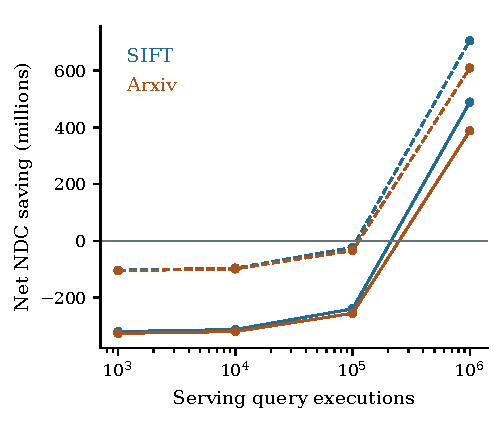
\includegraphics[width=\linewidth]{figures_v3/cost.pdf}
\caption{Modeled joint-error TCP net distance saving versus serving horizon. Cold history crosses zero later than cached history; fallback targets remain in the average.}
\label{fig:cost}
\Description{Net distance savings become positive only after the acquisition cost is amortized over a sufficiently long serving horizon.}
\end{figure}
